\chapter{自适应控制}\label{cp4}
\section{自适应控制概述}\label{4Aref}
\subsection{自适应控制的概念与缘由}
在设计系统时,我们常遇到下面情形:
\begin{enumerate}
  \item 待控制系统具有{\textbf{参数不确定性}}。
  
  \item 系统具有无法预测的{\textbf{参数摄动}}。
  
  \item 系统受到的{\bf 扰动特征}无法确知。
\end{enumerate}

为了抵御有确定上下界的参数摄动,首先考虑设计参数不变的反馈控制器,如图 \ref{adaptive_robust}(a) 所示。
  记闭环传递函数为$T$,有\[T=\frac{G(s)C(s)}{1+G(s)C(s)}\implies \frac{\diff T}{T}=\frac{1}{1+G(s)C(s)}\frac{\diff G(s)}{G(s)}\]
  可见,选取$C(s)$使得开环增益$|C(\mathrm{j}\omega)G(\mathrm{j}\omega)|$在我们感兴趣的频段足够大,那么模型对$G(s)$的变化(如参数摄动或不确定性)不敏感,并且由于增益接近于1,可认为$y=y^\ast$。
  只要$G(s)$的变化在一定范围内,就可以通过$C(s)$的设计来实现跟踪和稳定性目标。这就是所谓{\bf 鲁棒控制【robust (high gain) control】}。

但是,闭环并不是万能的:闭环后,有些系统输出受不确定性的影响会减小,有些反而增大;还有些系统无法用线性反馈控制器来控制。例子可见前言中参考文献6的例1.1-1.3,此处不录。

上面的设计,控制器参数是不变的。如果控制器参数能随着被控对象的变化而变化,以补偿不确定性带来的影响,可能收到更好的效果。
这样,我们就有下面的控制思想。
\begin{definition}[自适应控制器]
    \textbf{自适应控制器}是\textbf{结构固定}但具有\textbf{可变参数}的控制器,且带有一套自动调整参数的规则。
  \end{definition}
  其示意图如图 \ref{adaptive_robust}(b) 所示。
\begin{figure}[htbp]
  \centering
  \begin{subfigure}{0.4\textwidth}
    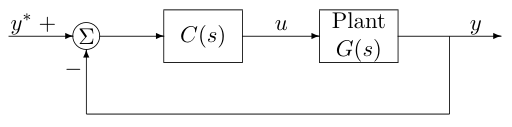
\includegraphics[width=1\linewidth]{figure/adaptive/robust.png} % width=...
    \caption{}
\end{subfigure}
  \begin{subfigure}{0.4\textwidth}
    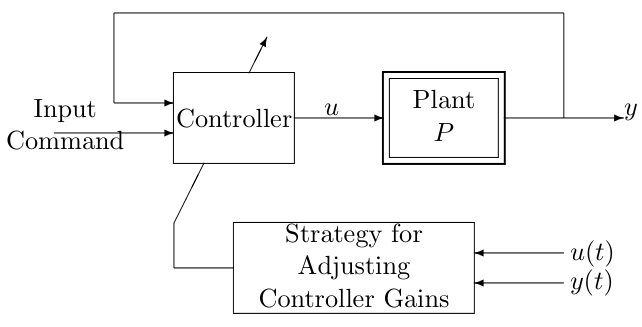
\includegraphics[width=1\linewidth]{figure/adaptive/adaptive_controller.png} % width=...
    \caption{}
\end{subfigure}
\caption{(a)鲁棒控制。(b)自适应控制。}
\label{adaptive_robust}
\end{figure}
  % \begin{description}
  %   \item[为什么采用自适应控制?]
    
  % \end{description}
鲁棒控制和自适应控制的对比如表 \ref{adaptive_robust_table}。也有将这两种思想结合,设计鲁棒自适应控制的,见 \ref{4Eref} 节。
\newpage
  \begin{table}[htbp]
    \vspace{5pt}
    \caption{自适应控制与鲁棒控制的对比}
    \label{adaptive_robust_table}
    \setcellgapes{4pt}
    \makegapedcells
    \small
    \centering
    \begin{tabular}{p{0.46\textwidth}|p{0.46\textwidth}}
      \hline
      {\bf 自适应控制(adaptive control)} & {\bf 鲁棒控制(robust control)} \\
      \hline
      对于处理慢变或不变的参数不确定性上更有优势 & 在处理扰动、快变参数和未建模动态上更有优势\\
      \hline
      随着自适应过程的进行,自适应控制器能不断提高系统性能 & 鲁棒控制器试图使系统维持恒定的性能 \\
      \hline
      自适应控制器几乎不需要对于位置参数的先验({\it a priori})信息 & 鲁棒控制器需要对于参数的界有合理的先验估计\\
      \hline
    \end{tabular}
  \end{table}

\begin{description}
  \item[自适应控制的一般设计步骤] 
  \begin{enumerate}
    \item 描述/刻画闭环系统的期望特性;
    \item 设计合适的控制律,其中包含可调参数;
    \item 求出调节这些参数的自适应律;
    \item 分析待控制变量的收敛性,应用控制律。
  \end{enumerate}
\end{description}
\subsection{自适应控制的类型}
\begin{enumerate}
      \item 非直接型(indirect): estimate plant parameters $\Rightarrow$ design
      controller parameters. The process model and possibly the disturbance
      characteristics are first determined. The controller parameters are
      designed on the basis of this information.
      
      \item 直接型(direct): directly design controller parameter. The controller
      parameters are changed directly without the characteristics of the process
      and its disturbance first being determined.
\end{enumerate}
\begin{figure}[htbp]
  \centering
  \begin{subfigure}{0.45\textwidth}
    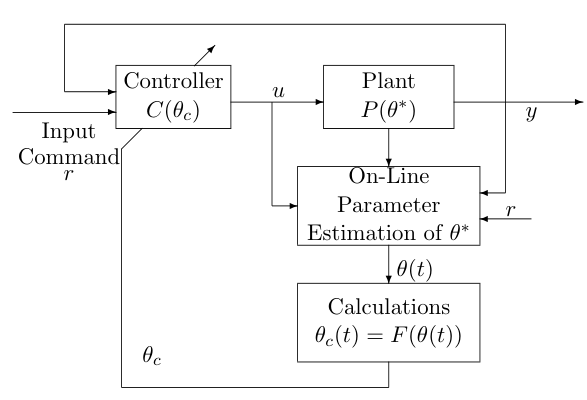
\includegraphics[width=1\linewidth]{figure/adaptive/indirect.png} % width=...
    \caption{}
\end{subfigure}
  \begin{subfigure}{0.45\textwidth}
    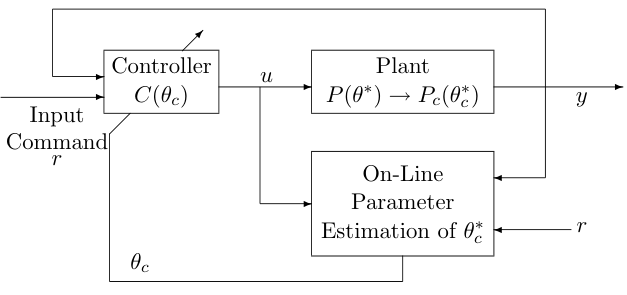
\includegraphics[width=1\linewidth]{figure/adaptive/direct.png} % width=...
    \caption{}
\end{subfigure}
\caption{(a)非直接型。(b)直接型。}
\label{direct_indirect}
\end{figure}
\subsection{自适应控制的常用手段}
  \begin{description}
    \item[增益调节(Gain Scheduling)]
    \begin{enumerate}
      \item 事先建立一张表(lookup table),建立测量得的指标(或称为辅助量测值,auxiliary measurements,可理解为工作点)与参数的对应关系,
      控制器的增益就随着工作点而变化。
      
      \item 优点:当系统动力学改变时,参数可根据这些改变迅速变化。
      
      \item 缺点:参数的更新是开环的,并不会根据系统的演变而“学到”新的信息。
    \end{enumerate}
  \end{description}

  \begin{center}
  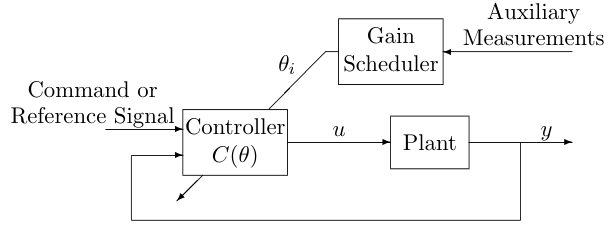
\includegraphics[scale=0.5]{figure/adaptive/gain_scheduling.png}
  \captionof{figure}{增益调节}
\end{center}
  \begin{description}
    \item[自调节控制器(Self-Tuning Controller,STC)]\index{自调节控制器(Self-Tuning Controller,STC)}
    \begin{enumerate}
      \item Controller parameters change in a predetermined fashion with the
      operating conditions.
      
      \item Performs simultaneous parameter identification and control.
      
      \item 利用确定性等价原理(Certainty Equivalence Principle)
    \end{enumerate}
  \end{description}
  \begin{center}
  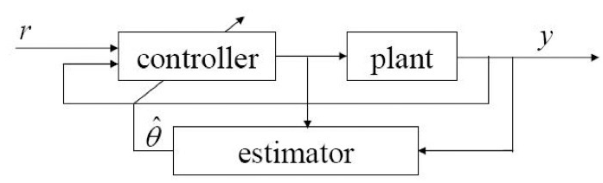
\includegraphics[scale=0.5]{figure/adaptive/stc.png}
  \captionof{figure}{自调节控制器}
\end{center}
  \begin{description}
    \item[模型参考自适应控制(Model Reference Adaptive Control, MRAC)]\index{模型参考自适应控制(Model Reference Adaptive Control, MRAC)}
    \begin{enumerate}
      \item Plant: containing unknown parameters and having a known structure.
      
      \item RM: specifying the desired output of the control system.
      
      \item Feedback control law: containing adjustable parameters.
      
      \item Adaptation mechanism: updating the adjustable parameters.
    \end{enumerate}
  \end{description}
\begin{figure}[htbp]
  \centering
  \begin{subfigure}{0.45\textwidth}
    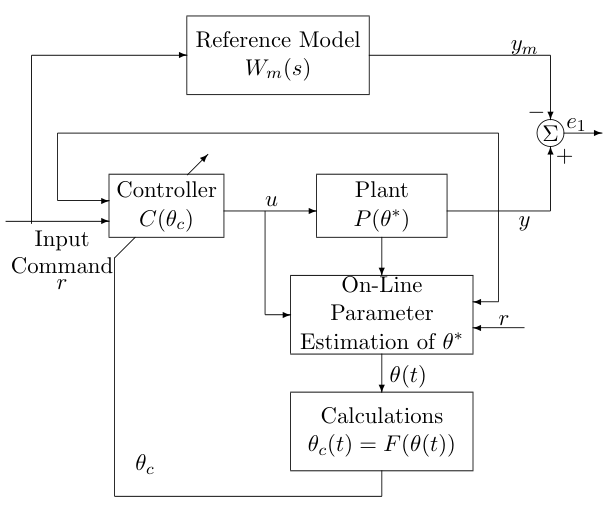
\includegraphics[width=1\linewidth]{figure/adaptive/indirect_MRAC.png} % width=...
    \caption{}
\end{subfigure}
  \begin{subfigure}{0.45\textwidth}
    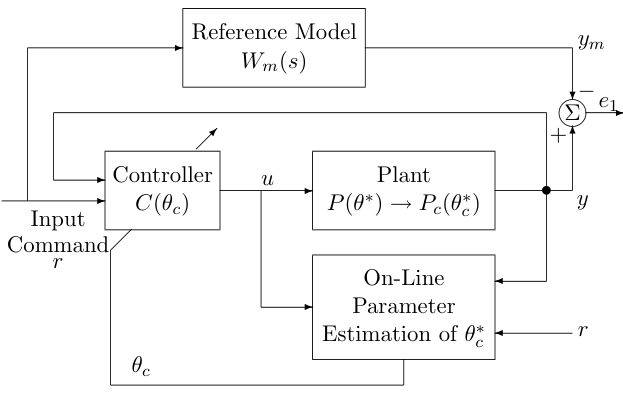
\includegraphics[width=1\linewidth]{figure/adaptive/direct_MRAC.png} % width=...
    \caption{}
\end{subfigure}
\caption{(a)非直接型MRAC。(b)直接型MRAC。}
\end{figure}